\usepackage[french]{babel}
\usepackage{
	amsmath,
	logochum,
	alveoli,
	n,
	hexagon,
	pgfplots,
	appendixnumberbeamer
}
\usepackage[
	backend=biber,
	autolang=none,
	style=authoryear,
	doi=false,
%	url=false,
	isbn=false
]{biblatex}

\setbeamercolor{fancy hexagon border}{fg=turquoisechum}
\usebeamercolor{fancy hexagon border}
\tikzset{
	fancyoct/.style={
		draw=fancy hexagon border.fg,
		line width=3.5mm,
		line join=round
	},
	fancyclip/.style={
		clip,
	},
	fancypict/.style={
		remember picture,
		overlay
	},
	titlegraphic/.style={
		above left,
		inner sep=0,
		opacity=0.7,
		xshift=0.0\pagewidth
	},
	fancyshade/.style={
		structure.fg,
		opacity=0.65
	}
}

\defbeamertemplate{background}{titlepage}[1][]{
	\begin{tikzpicture}[fancypict]
		\path [fancyoct] (current page.east)\hexagon{0.6\pageheight};
		\fill [fancyclip] (current page.east)\hexagon{0.6\pageheight};
		\node [titlegraphic] at(current page.south east) {\inserttitlegraphic};
		\fill [fancyshade] (current page.north west) rectangle (current page.south east);
	\end{tikzpicture}
}

\defbeamertemplate*{title page}{fancy}[1][]
{
  \vbox{}
  \vfill
  \begingroup
    \centering
    \begin{beamercolorbox}[sep=8pt,center,#1]{title}
      \usebeamerfont{title}\inserttitle\par%
      \ifx\insertsubtitle\@empty%
      \else%
        \vskip0.25em%
        {\usebeamerfont{subtitle}\usebeamercolor[fg]{subtitle}\insertsubtitle\par}%
      \fi%     
    \end{beamercolorbox}%
    \vskip1em\par
    \begin{beamercolorbox}[sep=8pt,center,#1]{author}
      \usebeamerfont{author}\insertauthor
    \end{beamercolorbox}
    \begin{beamercolorbox}[sep=8pt,center,#1]{institute}
      \usebeamerfont{institute}\insertinstitute
    \end{beamercolorbox}
    \begin{beamercolorbox}[sep=8pt,center,#1]{date}
      \usebeamerfont{date}\insertdate
    \end{beamercolorbox}
  \endgroup
  \vfill
}


\usetikzlibrary{
	datavisualization,
	external,
	shapes,
	shadows,
	matrix,
}
\usepgfplotslibrary{groupplots}

\tikzset{external/force remake}
\tikzsetexternalprefix{fig-pdf/}
%\tikzexternalize

\usecolortheme{chum}
\usefonttheme{structurebold}
\setbeamertemplate{title page}[fancy][left]
\setbeamertemplate{footline}[frame number]
\setbeamertemplate{footline}{
	\begin{tikzpicture}
		\fill[structure, opacity=0.2] (0,0) rectangle (\pagewidth, 1mm);
		\fill[structure] (0,0) rectangle
		({\pagewidth*((\insertframenumber)/(\inserttotalframenumber))}, 1mm);
		%\path (\pagewidth-8mm, 8mm) node [
		%	regular polygon,
		%	regular polygon sides=6,
		%	fill=bleuclairchum!30,
		%	shape border rotate=30,
		%	outer sep=3mm,
		%	inner sep=0pt,
		%	%minimum width=1.2cm
		%	minimum width=1.0cm
		%] {\insertframenumber/\inserttotalframenumber};
	\end{tikzpicture}
}
\setbeamertemplate{navigation symbols}{%
	%\insertslidenavigationsymbol%
	%\insertframenavigationsymbol%
	%\insertsectionnavigationsymbol%
	%\insertdocnavigationsymbol%
}
\setbeamercolor{structure}{fg=marinechum}
\setbeamercolor{subtitle}{use=structure, fg=title.fg!85}
\setbeamerfont{subtitle}{shape=\itshape, series=\mdseries}

\def\cmh{cmH\scalebox{0.7}{2}O}
\def\ox{O\scalebox{0.7}{2}}

\tikzset{
	postit/.style={
		fill=jaunechum,
		rounded corners,
		inner sep=3mm,
		drop shadow={
			opacity=0.3,
			fill=black
		},
		scale=0.8
	}
}

\pgfplotsset{
	compat=newest,
	tickwidth=1mm,
	every axis plot post/.append style={
		structure!60,
		line width=1pt,
	},
	every axis/.style={
		font=\tiny,
		fg!65,
		grid style={fg!30!bg, dotted},
		width=\textwidth,
		height=0.45\textheight,
		no markers,
		grid=both,
		minor x tick num=1,
		axis lines*=left,
		enlargelimits=false,
	},
}

\def\showwaveforms#1{%
	\begin{tikzpicture}[]

		\begin{groupplot}[
				group style={group size=1 by 2},
				xlabel=Temps (s),
			]

			\nextgroupplot[ymin=0,ylabel=Pression (\cmh)]
			\addplot [] table[x index=0, y index=2] {#1};

			\nextgroupplot[ylabel=Débit (l/m)]
			\addplot [] table[x index=0, y index=3] {#1};

		\end{groupplot}

	\end{tikzpicture}
}

\def\adaptcite#1{%
	\begingroup
	\vskip8pt
	\footnotesize
	\em{* Adapté de: \cite{#1}.}
	\endgroup
}

%\includeonly{frames/inspiration}

%%%%%%%%%%%%%
% Metadata
%%%%%%%%%%%%%

\title{Faux positifs et faux négatifs}
\subtitle{Failles de l'algorithme de déclenchement inspiratoire}
\author{\ninh}
\date{27 octobre 2021\\\scriptsize4\textsuperscript{e} vague de COVID-19}
\institute{\inhg\linebreak\chum}
\titlegraphic{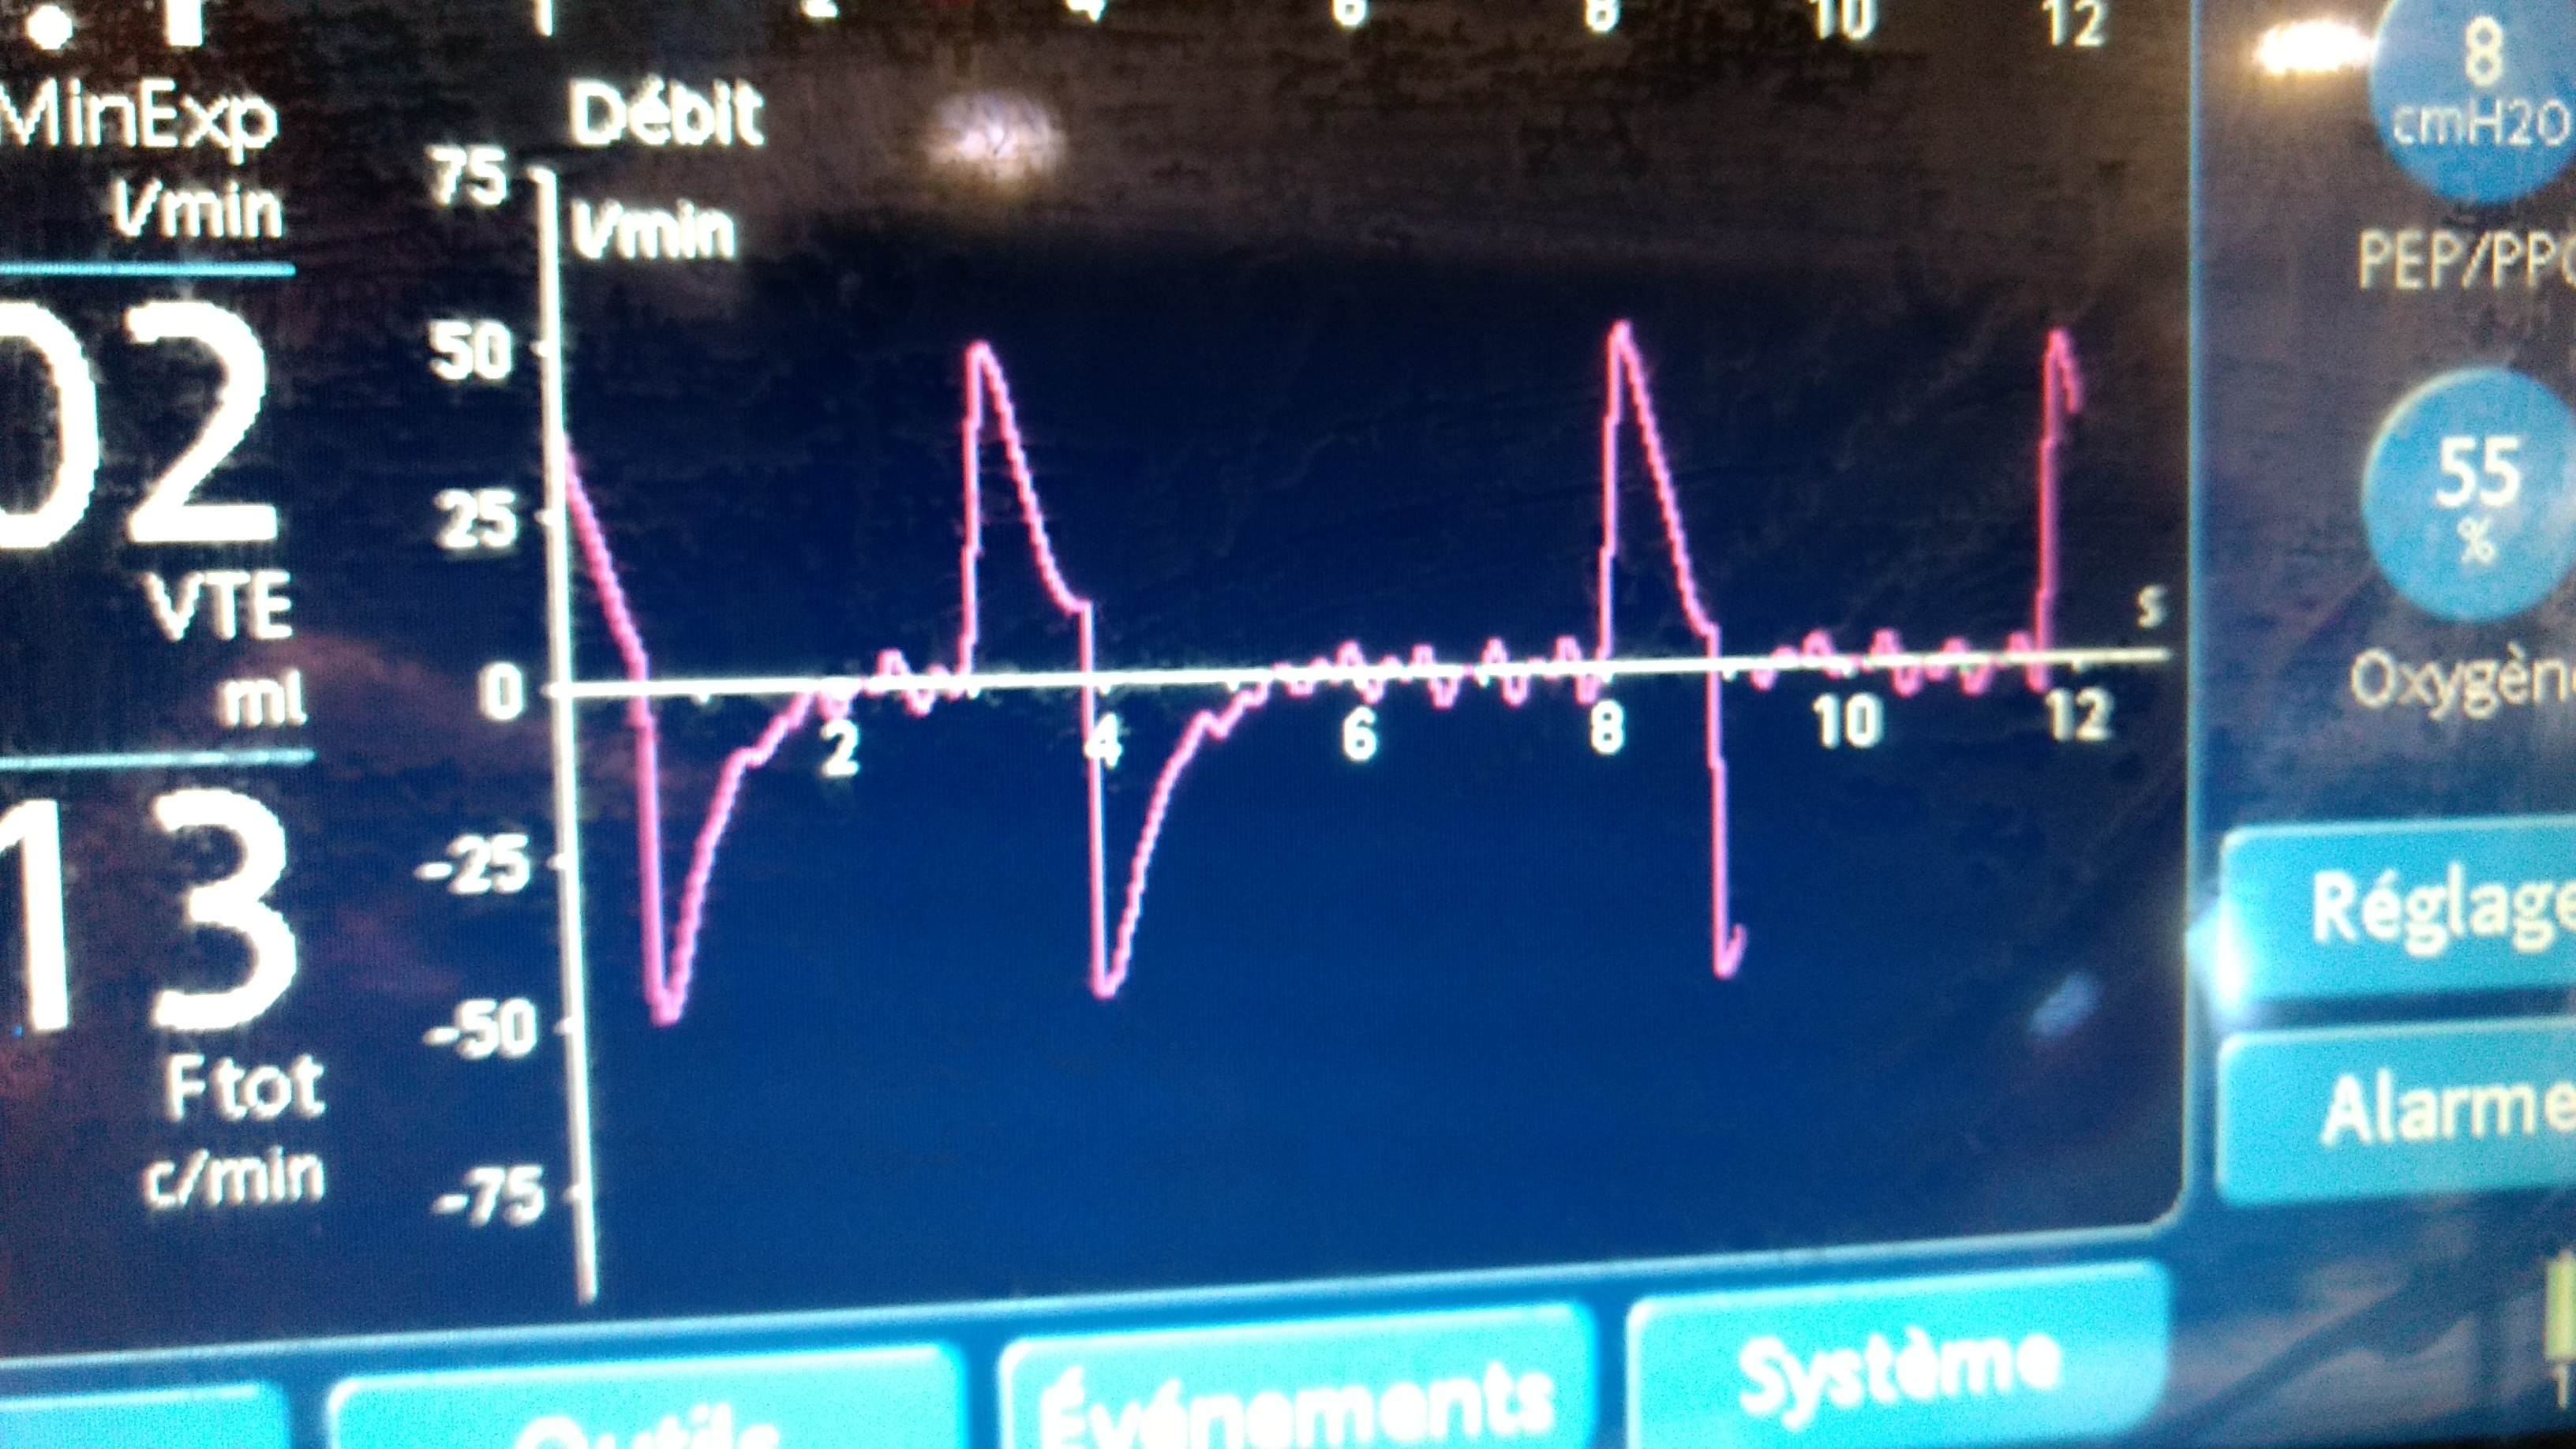
\includegraphics[height=\pageheight]{221.jpg}}
\addbibresource{bibliographie.bib}

%%%%%%%%%%%%%
% Document
%%%%%%%%%%%%%

\begin{document}

{
	\setbeamertemplate{background}[titlepage]
	\begin{frame}[plain]
	\maketitle
	\end{frame}
}


\section{Introduction}

\article{
	Comme toute chose conçue par l'hommes (ou la femme, d'ailleurs...),
	les algorithme de détection des efforts inspiratoire des ventilateurs
	ne sonts pas parfaits. Bien qu'appliqués sans erreurs par le
	microprocesseur du ventilateur, ses résultats comportent -comme pour
	n'importe quel test- leur lots de faux positifs et de faux négatifs.

	À votre avis, ces deux phénomènes sont-ils fréquents ou marginaux ?

	En avez vous déja observés ?

	Connaisses vous d'autres noms donnés à ces phénomènes ?

	Quelles peuvent êtres les conséquences de leur non-reconnaissance ?
}

%%%%%%%%%%%%%%%%%%%%%%%%%%%%%%%
\section{Faux négatifs}
%%%%%%%%%%%%%%%%%%%%%%%%%%%%%%%


\def\fauxneg{"data/Faux_négatifs/1555833401655-parsed.dat"}
\def\fauxnegbis{"data/Faux_négatifs/1555833504659-parsed.dat"}
\def\fauxnegtri{"data/Faux_négatifs/1558262528660-parsed.dat"}
\def\fauxnegcorige{"data/Faux_négatifs/1558262056661-parsed.dat"}

\tikzset{
	annot/.style={
		red,
		<-,
		draw,
		thick,
		circle,
		minimum width=30,
		inner sep=0,
		yshift=-2,
		font=\normalfont
	}
}

\begin{frame}{Qu'est-ce qui cloche ?}
	\begin{tikzpicture}[]

		\begin{groupplot}[
				group style={
					group name=my group,
					group size=1 by 3,
				},
				xmax=16,
				every axis style/.append style={
					minor x ticks num=3,
					grid=both,
				}
				height=0.5\textheight,
				xlabel=Temps (s),
				anchor=center,
				at={(0,0)}
			]

			\nextgroupplot[
				ymin=0,
				ylabel=Pression (\cmh),
				height=0.32\textheight
			]

			\addplot [] table[x index=0, y index=2] {\fauxnegtri};

			\nextgroupplot[ylabel=Débit (l/m), height=0.45\textheight]
				\addplot [] table[x index=0, y index=3] {\fauxnegtri};
				\coordinate (myanchor) at(12.75,0) ;
				\node<2,3>[annot] at (4,0) {};
				\node<2,3>[annot] at (11.8,0) {};

			\only<3->{
				\nextgroupplot[ylabel=EADI (mcv), height=0.31\textheight]
					\addplot[] table[x index=0, y index=5] {\fauxnegtri};
					\coordinate (x1) at(axis cs:3.05,0);
					\coordinate (x2) at(axis cs:8,0);
					\coordinate (x3) at(axis cs:8.75,0);
			}

		\end{groupplot}

		\only<4-5>{
			\draw [red, dashed] (x1) -- ++(0, \textheight-66pt);
		}
		
		\only<5>{
			\draw [red, dashed] (x2) -- ++(0, \textheight-66pt) coordinate(c1);
			\draw [red, dashed] (x3) -- ++(0, \textheight-66pt) coordinate(c2);
			\draw [<->, red] (c1) -- (c2) node[midway, above] {0,75 s};
		}

		\node <6>[
			postit,
		] at (myanchor) {
			\begin{tabular}{l @{\ :\ \ } r @{ } >{\footnotesize}l }
				Volume courant   & 450 & ml \\
				PEP              & 5   & \cmh \\
				F resp.          & 12  & resp/min \\
				Conc. \ox        & 35  & \% \\
				Pente tps insp.  & 0   & s \\
				Durée de plateau & 0   & s \\
				Décl. en débit   & 0   & l/min \\
				Ti               & 0,5 & s
			\end{tabular}
		};
	\end{tikzpicture}
\end{frame}

\begin{frame}{Équation du mouvement de l'air}
	\begin{align*}
		\uncover<1->{P_{musc} + P_{vent} &= P_{el} + P_{res}}  \\
		\uncover<2>{P_{musc} + P_{vent} &= \frac{Volume - CRF}{Compliance}  + Resist. \times \dot V}
	\end{align*}
\end{frame}

\def\tripledown{$\downarrow\downarrow\downarrow$}
\tikzset{
	pres/.style={
		draw,
		circle,
		inner sep=2pt
	},
	negpres/.style={
		pres,
		node contents=-,
		label=[pres]-120:-,
		label=[pres]-60:-,
	},
	pospres/.style={
		pres,
		node contents=+,
		label=[pres]120:+,
		label=[pres]60:+,
	},
	flowdown/.style={
		node contents={$\downarrow$},
		inner sep=1pt
	},
	bflowdown/.style={
		node contents={$\downarrow$},
		label=100:$\downarrow$,
		label=80:$\downarrow$,
		inner sep=1pt
	},
	bflowup/.style={
		node contents={$\uparrow$},
		label=-100:$\uparrow$,
		label=-80:$\uparrow$,
		inner sep=1pt
	},
	flowup/.style={
		node contents={$\uparrow$},
		inner sep=1pt
	},
	flowlabel/.style={
		pin=[pin distance=1cm]right:$\frac{\Delta P}{R}$
	}
}

\begin{frame}{Comment respirer...}{En 4 étapes \em{faciles} !}
	\centering
	\begin{tikzpicture}

		\pic<1-2>(A) {assini={alveoli radius=1.15cm}};

		\uncover<2>{
			\node[below, label=0:$P_{musc.}$] at(A-alveoli.south) {\tripledown};
		}

		\uncover<3->{
			\pic<+->(A) {assini={previous volume radius=1.15cm}};
			\node[below, label=0:$P_{musc.}$] at(A-alveoli.south) {\tripledown};

			\node[above] at(A-alveoli.south) {$\uparrow$};
			\node[above, rotate=45, label={[absolute, label distance=3mm]-0:$P_{el}$}] (PELR) at(A-alveoli.-45) {$\uparrow$};
			\node[above, rotate=-45] at(A-alveoli.-135) {$\uparrow$};
		}

		\uncover<4->{\draw (A-previous) node [negpres];}

		\uncover<5>{\draw (A-bronchus) node [flowdown];}

		\uncover<6->{
			\draw (A-bronchus.north) node [pospres, above];
			\draw (A-bronchus) node [bflowdown];
		}
	\end{tikzpicture}
\end{frame}

\begin{frame}{Quand ça ne marche pas comme prévu ...}
	{En 4 étapes moins faciles ...}
	\centering

	\begin{tikzpicture}[
		]
		\pic (A) at(0,0) {assini={ previous volume radius=1.15cm, }};

		%%%%%%%%%%
		% Labels %
		%%%%%%%%%%

		\uncover<+>{
			\node [pin={0:Vol. act.}] at(A-alveoli.-15) {};
			\node [pin=0:CRF] at(A-previous.0) {};
		}


		%%%%%%%%%%%%%%%%%%
		% Elastic recoil %
		%%%%%%%%%%%%%%%%%%
		\uncover<+->{
			\node[above] at(A-alveoli.south) {$\uparrow$};
			\node[above, rotate=45] (PELR) at(A-alveoli.-45) {$\uparrow$};
			\node[above, rotate=-45] at(A-alveoli.-135) {$\uparrow$};
		}

		\uncover<+->{
			\draw (A-previous) node [pospres, rotate=180];
		}

		\uncover<+>{
			\draw (A-bronchus) node [bflowup];
		}

		\uncover<+->{
			\node[below, label=0:$P_{musc.}$] at(A-alveoli.south) {\tripledown};
			\draw (A-bronchus) node [flowup];
		}

	\end{tikzpicture}

\end{frame}

\begin{frame}{Caractéristiques des non-déclencheur}
\centering
\rowcolors{3}{vertchum!15}{white}
	\begin{tabular}{l >{\scriptsize}l c c}
	\hline
	\rowcolor{vertchum!50}
	Faux négatifs          &          & < 10 \% & > 10 \% \\
	\rowcolor{vertchum!50}
	Nombre de patients     &          & 51      & 11 \\
	\hline
	Hommes                 & (\%)     & 71      & 100 \\
	MPOC                   & (\%)     & 20      & 55 \\
	pH                     &          & 7,44    & 7,49\\
	Bicarbonates           & (mmol/l) & 24      & 28 \\
		Volume courant       & (ml)     & 500     & 650 \\
	Fréq. du ventilateur   & (/min)   & 25      & 18 \\
	Seuil de déclenchement & (l/min)  & 1,0     & 1,5 \\
	Pressions de pointe    & (\cmh)   & 20      & 25 \\
	Aide inspiratoire      & (\cmh)   & 15      & 18\\
	\hline
\end{tabular}

	\adaptcite{thille_patient-ventilator_2006}

\end{frame}

\begin{frame}{Magie du NAVA ...}
	\begin{tikzpicture}[]

		\begin{groupplot}[
				group style={
					group name=my group,
					group size=1 by 3,
				},
				xmax=16,
				height=0.5\textheight,
				xlabel=Temps (s),
				anchor=center,
				at={(0,0)}
			]

			\nextgroupplot[ymin=0,ylabel=Pression (\cmh), height=0.35\textheight]
			\addplot [] table[x index=0, y index=2] {\fauxnegcorige};

			\nextgroupplot[ylabel=Débit (l/m), height=0.42\textheight]
			\addplot [] table[x index=0, y index=3] {\fauxnegcorige};
			\coordinate (myanchor) at(12.5,0);

			\nextgroupplot[ylabel=EADI (mcv), height=0.35\textheight]
			\addplot [] table[x index=0, y index=5] {\fauxnegcorige};

		\end{groupplot}

			\node <2>[postit] at (myanchor) {
				\begin{tabular}{l @{\ :\ \ } r @{ } >{\footnotesize}l }
					PEP            & 5   & \cmh \\
					Conc. \ox      & 35  & \% \\
					Décl. en débit & 0   & l/min \\
					Niveau NAVA    & 3,8 & \cmh/uV \\
					Trigger Edi    & 0,5 & uV
				\end{tabular}
			};
	\end{tikzpicture}
\end{frame}


%%%%%%%%%%%%%%%%%%%%%%%%%%%%%%%
\section{Faux positif}
%%%%%%%%%%%%%%%%%%%%%%%%%%%%%%%

\def\fauxpos{"data/Faux_positifs/1628779222908-parsed.dat"}
\begin{frame}{Qu'est-ce qui cloche ?}
	\begin{tikzpicture}[]

		\begin{groupplot}[
				group style={
					group size=1 by 2,
				},
				xlabel=Temps (s),
			]

			\nextgroupplot[ymin=0,ylabel=Pression (\cmh)]
			\addplot [] table[x index=0, y index=2] {\fauxpos};
			\coordinate (myanchor) at(22,0);

			\nextgroupplot[ylabel=Débit (l/m)]
			\addplot [] table[x index=0, y index=3] {\fauxpos};

		\end{groupplot}
		\node <2>[postit] at (myanchor) {
			\begin{tabular}{l @{\ :\ \ } r @{ } >{\footnotesize}l }
				PEP                & 7    & \cmh\\
				Niv. AI sur PEP    & 8    & \cmh\\
				Décl. en débit     & 1    & l/min\\
				Pentetps insp. (s) & 0,15 & s\\
				Fin d'insuff.      & 30   & \% \\
			\end{tabular}
		};

	\end{tikzpicture}
\end{frame}

%\def\fauxposcorige{"data/Faux_positifs/1628779150902-parsed.dat"}
\def\fauxposcorige{"data/Faux_positifs/1628779169421-parsed.dat"}

\begin{frame}{Après un petit ajustement ...}
	\begin{tikzpicture}[]

		\begin{groupplot}[
				group style={
					group size=1 by 2,
				},
				xlabel=Temps (s),
			]

			\nextgroupplot[ymin=0,ylabel=Pression (\cmh)]
				\addplot [] table[x index=0, y index=2] {\fauxposcorige};
				\coordinate (formulae) at(17, 12);

			\nextgroupplot[ylabel=Débit (l/m)]
				\addplot [] table[x index=0, y index=3] {\fauxposcorige};
				\coordinate (myanchor) at(22,40);
				\coordinate (x1) at(12.0, \pgfkeysvalueof{/pgfplots/ymin});
				\coordinate (x2) at(12.7, \pgfkeysvalueof{/pgfplots/ymin});

		\end{groupplot}

		\only<2-3>{
			\draw [dashed, red] (x1) -- ++(0,\textheight-103pt) coordinate (c1);
			\draw [dashed, red] (x2) -- ++(0,\textheight-103pt) coordinate (c2);
			\draw [<->, red] (c1) -- (c2) node [midway, above] {0,7 s} ;
		}
		\node <3>[postit, scale=1] at(formulae) {$\frac{1}{0,7 s} = 86 /min$};

		\node <4>[postit] at ([yshift=4mm]myanchor) {
			\begin{tabular}{l @{\ :\ \ } r @{ } >{\footnotesize}l }
				PEP                & 7    & \cmh\\
				Niv. AI sur PEP    & 8    & \cmh\\
				Décl. en pression  & -2   & \cmh\\
				Pentetps insp. (s) & 0,15 & s\\
				Fin d'insuff.      & 30   & \% \\
			\end{tabular}
		};

	\end{tikzpicture}
\end{frame}

\begin{frame}{Caractéristiques des autodéclencheur}
	\centering
	\def\mytblcolor{grischum}
	\rowcolors{3}{\mytblcolor!25}{white}

	\def\pa{p < .01}
	\def\pb{p < .05}
	\def\urvasc{dyne$\cdot$s/cm\textsuperscript{5}}
	\begin{tabular}{l >{\scriptsize}l c c >{\scriptsize}c}
		\hline
		\rowcolor{\mytblcolor!70}
		                              &          & FP   & Non-FP & \\
		\rowcolor{\mytblcolor!70}
		                              &          & n=23 & n=81   & \\
		\hline
		Résistances voies respi.      & \cmh/l/s & 8.5  & 10     & \pa \\
		Constante de temps            & s        & .41  & .49    & \pa \\
		Ratio cardiothoracique        & \%       & 61   & 58     & \pb \\
		Débit cardiaque               & l/min    & 5.5  & 4.2    & \pa \\
		Index cardiaque               & l/min/m² & 3,38 & 2,62   & \pa \\
		Volume d'éjection             & ml       & 60   & 48     & \pa \\
		Pression veineuse centrale    & mmHg     & 9,2  & 7,2    & \pa \\
		Pres. cap. plum . bloq.       & mmHg     & 10.9 & 8.7    & \pb \\
		Résist. vasc. systémique      & \urvasc  & 1278 & 1608   & \pa \\
		Résist. vasc. pulmonaire      & \urvasc  & 151  & 206    & \pa \\
		\hline
	\end{tabular}

	\adaptcite{imanaka_autotriggering_2000}
\end{frame}

\begin{frame}
\frametitle{Références}
	\printbibliography{}
\end{frame}

\appendix

%%%%%%%%%%%%%%%%%%%%%%%%%%%%%%%
\section{Contrôle de la respiration}
%%%%%%%%%%%%%%%%%%%%%%%%%%%%%%%

\begin{frame}{Contrôle de la respiration}
	\centering
	\begin{tikzpicture}[
			outer sep=2mm,
			bulbe rachidien/.style={
			draw,
			circle,
			align=flush center
		}
		]

		\node [bulbe rachidien] (cr) {Bulbe\\rachidien};

		\node (co2) at(160:4) {$CO_2$, $O_2$, pH};
		\node [align=flush center] (cortex) at(200:4) {Stress,\\douleur,\\temp.};
		\node (freq) at(20:4) {Freq. (Ti et Te)};
		\node (vol) at(-20:4) {Vol. (force)};

		\node [yshift=1.5cm] (E) at (co2) {\structure{Entrée}};
		\node [yshift=1.5cm] (S) at (freq) {\structure{Sortie}};
		\path (E) -- (S) node [midway] (C) {\structure{Contrôle}} ;

		\draw [->] (E) -- (C);
		\draw [->] (C) -- (S);
		\draw [->] (co2) -- (cr);
		\draw [->] (cortex) -- (cr);
		\draw [->] (cr) -- (freq);
		\draw [->] (cr) -- (vol);
	\end{tikzpicture}
\end{frame}

\begin{frame}{Contrôle de la respiration}
	\centering
	\begin{tikzpicture}[
			pin distance=1ex,
			every pin edge/.style={
				very thick
			},
			cpupin/.style={
				inner sep=0
			},
			cpu/.style={
				thick,
				draw, 
				rounded corners, 
				outer sep=1mm,
				minimum size=2cm,
				fill=black!70,
				text=white,
				inner sep=3mm,
				font=\bf,
				append after command={
					(CPU.150) -- (CPU.30) 
					foreach \dist in {1, 2, ..., 9}{%
						node[cpupin, pos=0.1*\dist, pin={90:{}} ] (P\dist) {}
						}
						(CPU.-150) -- (CPU.-30) 
						foreach \dist in {1, 2, ..., 9}{%
							node[cpupin, pos=0.1*\dist, pin={-90:{}} ] (P\dist) {}
							}
						}
					},
					arklink/.style={
						bend left=60,
						->,
						looseness=1.5,
						thick
					}
				]

		\node [cpu] (CPU) {Microprocesseur};
		\node [below=1cm, align=flush center] (E) at(CPU.south) {Débit\\Pression};
		\draw[arklink] (CPU.east) to (E.east);
		\draw[arklink] (E.west) to (CPU.west);
		%\node [left=1cm] (E) at(CPU.west) {Débit, Pression};
		%\node [right=1cm] (O) at(CPU.east) {Débit, Pression};
		%\draw [->] (E) -- (CPU);
		%\draw [->] (CPU) -- (O);


	\end{tikzpicture}
\end{frame}

\tikzset{
	circuit/.style={
		decorate, 
		double distance=4mm,
		decoration={
			snake, 
			pre length=4mm,
			post length=4mm,
			segment length=2.5mm,
			amplitude=.5mm,
		}
	},
	y/.pic={
		\draw[double distance=4mm] 
		(.5,0) -- ++(180:0.5) -- ++(+135:0.5) -- ++(180:0.2) coordinate (-C1)
		(.5,0) -- ++(180:0.5) -- ++(-135:0.5) -- ++(180:0.2) coordinate (-C2)
		;
		\coordinate (-PT) at(0.5,0);
	}
}

\begin{frame}{Déclenchement par débit}
	\begin{columns}
		\begin{column}{0.5\textwidth}
			\centering
			\begin{tikzpicture}[
					label distance=1.5mm
					]
				\pic (y){y};
				\draw [circuit] (y-C1) -- ++(-4cm,0) node[midway, label=above:Isnpi.] {$\rightarrow$};
				\draw [circuit] (y-C2) -- ++(-4cm,0) node[midway, label=below:Expi.] {$\leftarrow$};
				\node [right] at(y-PT) {Pt};
				\node [left, font=\footnotesize] at(y-PT) {$\leftrightarrow$};
			\end{tikzpicture}
		\end{column}
		\begin{column}{0.5\textwidth}
			\centering
			$\dot V_{I} - \dot V_{E} = \dot V_{pt}$
		\end{column}
	\end{columns}
\end{frame}


\end{document}
